\documentclass[12pt]{article}
\usepackage[paper=letterpaper, margin=0.8in]{geometry}

%% The graphicx package provides the includegraphics command.
\usepackage{graphicx}
%% The amssymb package provides various useful mathematical symbols
\usepackage{amssymb}
%% The amsthm package provides extended theorem environments
%% \usepackage{amsthm}
%% fix strange gensymb error
\usepackage{textcomp}
%% symbols, especially degree
\usepackage{gensymb}
%% scientific units
\usepackage{siunitx}
%% line spacing
\usepackage{setspace}
\doublespacing
%% put figures at the end
%\usepackage[nomarkers]{endfloat}
%% allow hyperlinks
%\usepackage{hyperref}
%% color comments
\usepackage{soul}
\usepackage{color}
%% left justification in tables
\usepackage{array}
\newcolumntype{P}[1]{>{\raggedright\arraybackslash}p{#1}}
%%references
\usepackage[round]{natbib}
%%landscape orientation
\usepackage{pdflscape}


%% The lineno packages adds line numbers. Start line numbering with
%% \begin{linenumbers}, end it with \end{linenumbers}. Or switch it on
%% for the whole article with \linenumbers after \end{frontmatter}.
\usepackage{lineno}

\begin{document}

\title{Carry-over effects of larval microclimate on the transmission potential of a mosquito-borne pathogen\\
\large Supplemental Figures}
\author{
		Michelle V. Evans\\
		\and
		Justine C. Shaiu\\
		\and
		Nicole Solano\\
		\and
		Melinda A. Brindley\\
		\and
		John M. Drake\\
    \and
    Courtney C. Murdock
		}
\date{}
\maketitle

\newpage
\begin{figure}
\centering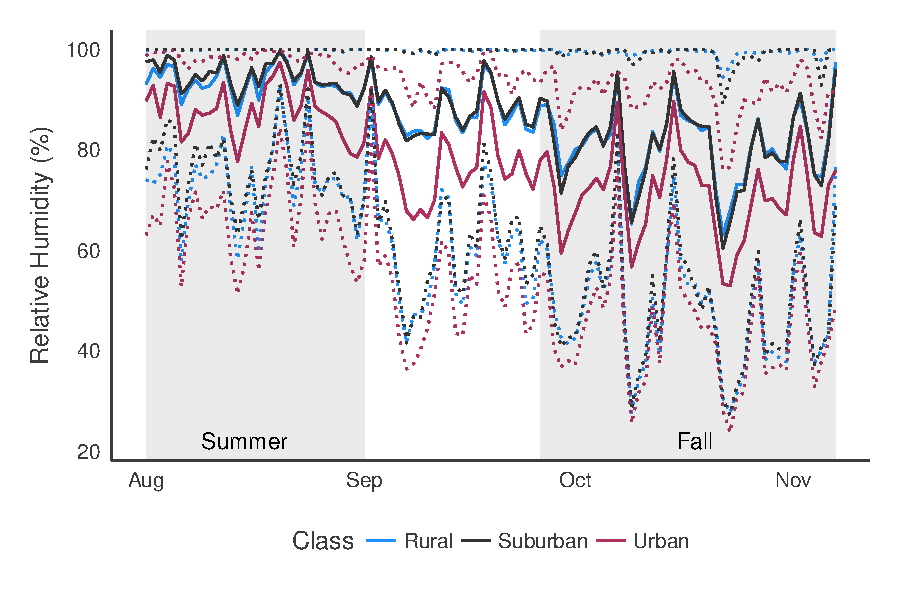
\includegraphics[width=0.9\linewidth]{relativeHumiditySupp1.pdf}
\caption{Supplementary Figure 1. Relative humidity across season and land class. The solid line represents the mean temperature across trays in each land class. The dotted lines represent the mean minimum and maximum relative humidity across trays in each land class.}
\end{figure}

\end{document}
